\documentclass[11pt]{article}
\linespread{1.5} 
\usepackage{graphicx,epstopdf,subfigure,mathtools,mathrsfs, arydshln, amsmath, amssymb} 
\usepackage[font=small,labelfont=bf]{caption}
\usepackage{float}
\usepackage{authblk, enumitem}
\usepackage[title]{appendix}
\PassOptionsToPackage{usenames,dvipsnames}{xcolor}
\usepackage[usenames,dvipsnames]{xcolor}
\usepackage[margin=1in]{geometry}
\usepackage[normalem]{ulem}

\usepackage{amsfonts}
\usepackage{hyperref}
\usepackage[round]{natbib}

\graphicspath{{Glotzer/}}

\hypersetup{
    colorlinks=false,
    pdfborder={0 0 0},
}
\newcommand{\new}[1]{\color{blue}#1\normalcolor}
\newcommand{\red}[1]{\color{red}#1\normalcolor}
\newcommand{\delete}[1]{}
\newcommand{\change}[1]{\color{black}#1\normalcolor}
\newcommand{\rev}[1]{\color{black}#1\normalcolor}

% VECTOR AND MATRIX NOTATION
\newcommand{\V}[1]{\boldsymbol{#1}}                 % vector notation
\newcommand{\M}[1]{\boldsymbol{#1}}
\global\long\def\norm#1{\left\Vert #1\right\Vert }
\newcommand{\Tot}[1]{#1^\text{(Tot)}}
\global\long\def\Dt{\partial_t}
\global\long\def\Dx{\partial_x}
\global\long\def\Koff{K^\text{off}}
\global\long\def\Kon{K^\text{on}}
\global\long\def\koff{k^\text{off}}
\global\long\def\koffb{\bar{k}^\text{off}}
\global\long\def\kon{k^\text{on}}
\global\long\def\Kae{K_\text{AE}}
\global\long\def\Kme{K_\text{ME}}
\global\long\def\Kem{K_\text{EM}}
\global\long\def\Kfb{K_\text{fb}}

\title{Modeling dynamics of AIR-1, ECT-2, and myosin in polarity establishment and cytokinesis \vspace{-0.5 cm}}
%\title{Mathematical appendix: \\ Oligomerization and feedback on membrane recruitment stabilize PAR-3 asymmetries in \emph{C.\ elegans} zygotes}
\author{Ondrej Maxian and Michael Glotzer \vspace{-0.75 cm}}

\begin{document}
\maketitle

\begin{abstract}
In early \emph{Caenorhabditis elegans} embryos, contractility is partially controlled by the protein ECT-2, which acts through the GTPase RhoA to activate myosin and cortical flows. Centrosomal Aurora A (AIR-1) locally inhibits ECT-2, leading to larger-scale myosin flows that amplify ECT-2 asymmetries in both polarization and cytokinesis (Longhini and Glotzer, 2022). In this study, we construct a mathematical model to determine how dynamics of ECT-2 during polarization and cytokinesis are shaped by the AIR-1 cue and myosin flows. Our model, which combines a two-dimensional description of the AIR-1 profile (on the embryo cross section) with a one-dimensional description of the cortex (boundary of the cross section) demonstrates that myosin-based amplification of local AIR-1 activity is necessary to explain the cortical distribution of ECT-2 during cytokinesis. Applying the same model to polarization shows how myosin-based recruitment of ECT-2 combines with a short ECT-2 residence time to yield robust symmetry breaking.
\end{abstract}

\section{Introduction}
The anterior-posterior axis of the nematode \emph{C.\ elegans} is determined in the zygote, shortly after the egg is fertilized.  The position of sperm entry dictates the posterior pole. This event triggers myosin-dependent, anterior-directed cortical flows that facilitate the segregation of anterior and posterior PAR proteins into distinct domains \citep{munro2004cortical, lang2017proteins, gross2019guiding}.

Recent studies implicated Aurora A kinase, AIR-1, as a crucial factor required to initiate these cortical flows \citep{klinkert2019aurora,kapoor2019centrosome, longhini2022aurora}. AIR-1 associates with the sperm centrosome, which is the sperm-derived structure that promotes polarity establishment \citep{hannak2001aurora}. Recent work from our lab \citep{longhini2022aurora} showed that AIR-1 impacts dynamics on the cortex by inhibiting the Rho GEF ECT-2. Specifically, ECT-2 dissociates from the posterior membrane in an AIR-1 dependent manner, and it contains a consensus site for AIR-1 that is required for AIR-1 responsiveness. During polarization, ECT-2 exhibits posterior depletion and anterior enrichment, a pattern of accumulation that requires cortical myosin flows. However, unlike the anterior PAR proteins, which have residence times on the order of one hundred seconds \citep{robin2014single}, ECT-2 cannot be strongly advected, as it exchanges rapidly between the cytoplasm and the cortex on timescales of a few seconds, appearing to preferentially bind to the cortex at myosin-enriched sites \citep{longhini2022aurora}. Consequently, it remains unclear how a short residence time, preferential recruitment by myosin, and weak advection by cortical flows, could combine to generate the observed ECT-2 asymmetries during polarization. 

We also previously showed that a similar set of events occur upon anaphase onset, coincident with cytokinesis \citep{longhini2022aurora}. At first glance, these events appear quite different, as by the time cytokinesis is reached, the centrosomes have matured,  accumulated much more \mbox{AIR-1}, and moved farther away from the cortex. Yet we reported a strong, ultra-sensitive dependence between the distance of the centrosome from the nearest cortical domain and the amount of cortical ECT-2 at that site; proximal centrosomes correlated with a reduction in cortical ECT-2. Because cytokinesis requires myosin, it is not possible to experimentally test how the AIR-1 signal shapes the ECT-2 distribution through myosin during cytokinesis, thus leaving open the question of whether the same mechanism that drives polarization is also responsible for the ultra-sensitive centrosome position/ECT-2 accumulation relationship in cytokinesis.

In this study, we use a mathematical model to test whether the same underlying circuitry could explain the dynamics of both of these phases. Because our data is more abundant during cytokinesis, we choose to begin there. We first show that the simplest model, in which AIR-1 diffuses from the centrosomes to the cortex, where it locally inhibits ECT-2, is insufficient to explain the ultra-sensitivity we observe in our previous data \citep[Fig.~7A]{longhini2022aurora}. Incorporating ECT-2 mediated activation of myosin (through Rho), plus preferential recruitment of ECT-2 by myosin, and advection of both myosin and ECT-2 through flow, then gives a closer match to our experimental data. 

Having conditioned the model (which ultimately has two unknown parameters) on cytokinesis, we then apply it to polarization \emph{without changing the parameters that govern the dynamics.} In doing so, we demonstrate that the observed dynamics of polarization and (centralspindlin-independent) cytokinesis can be explained by the same underlying model. In the context of polarization, we specifically assert that the preferential recruitment by myosin, rather than a longer bound lifetime of ECT-2, is what gives rise to the effective advection observed experimentally. 

\subsection{Basic model of contractility}

\section{Dynamics of polarization}
Having used cytokinesis, where we have more quantitative measurements of ECT-2 accumulation, to fit our model, we now proceed to look at polarization, where we are more interested in qualitative phenomena. In the absence of PAR proteins, it is known that the AIR-1/ECT-2 signal from the centrosomes leads to transient clearing of myosin from the posterior pole, and that the myosin profile reverts back to a uniform state after the centrosomes move towards the cell equator \citep[Fig.~2E]{gross2019guiding}. But is the transient clearing driven by the same underlying circuitry as cytokinesis? To answer this, we apply our model from cytokinesis to polarization, without changing any of the underlying parameters except for the AIR-1 signal.

\subsection{The centrosome distance determines the strength of polarization \label{sec:airpol}}
In cell polarization, \emph{both} centrosomes sit very close to the posterior cortex (about 1 $\mu$m away \citep{cowan2004centrosomes}). The centrosomes have a smaller size (about 0.2 $\mu$m). They also contain substantially less total AIR-1; here we assume that the amount scales with the area, so that the amount of AIR-1 on each centrosome during polarization is 1\% of that for cytokinesis. 

\begin{figure}
\centering
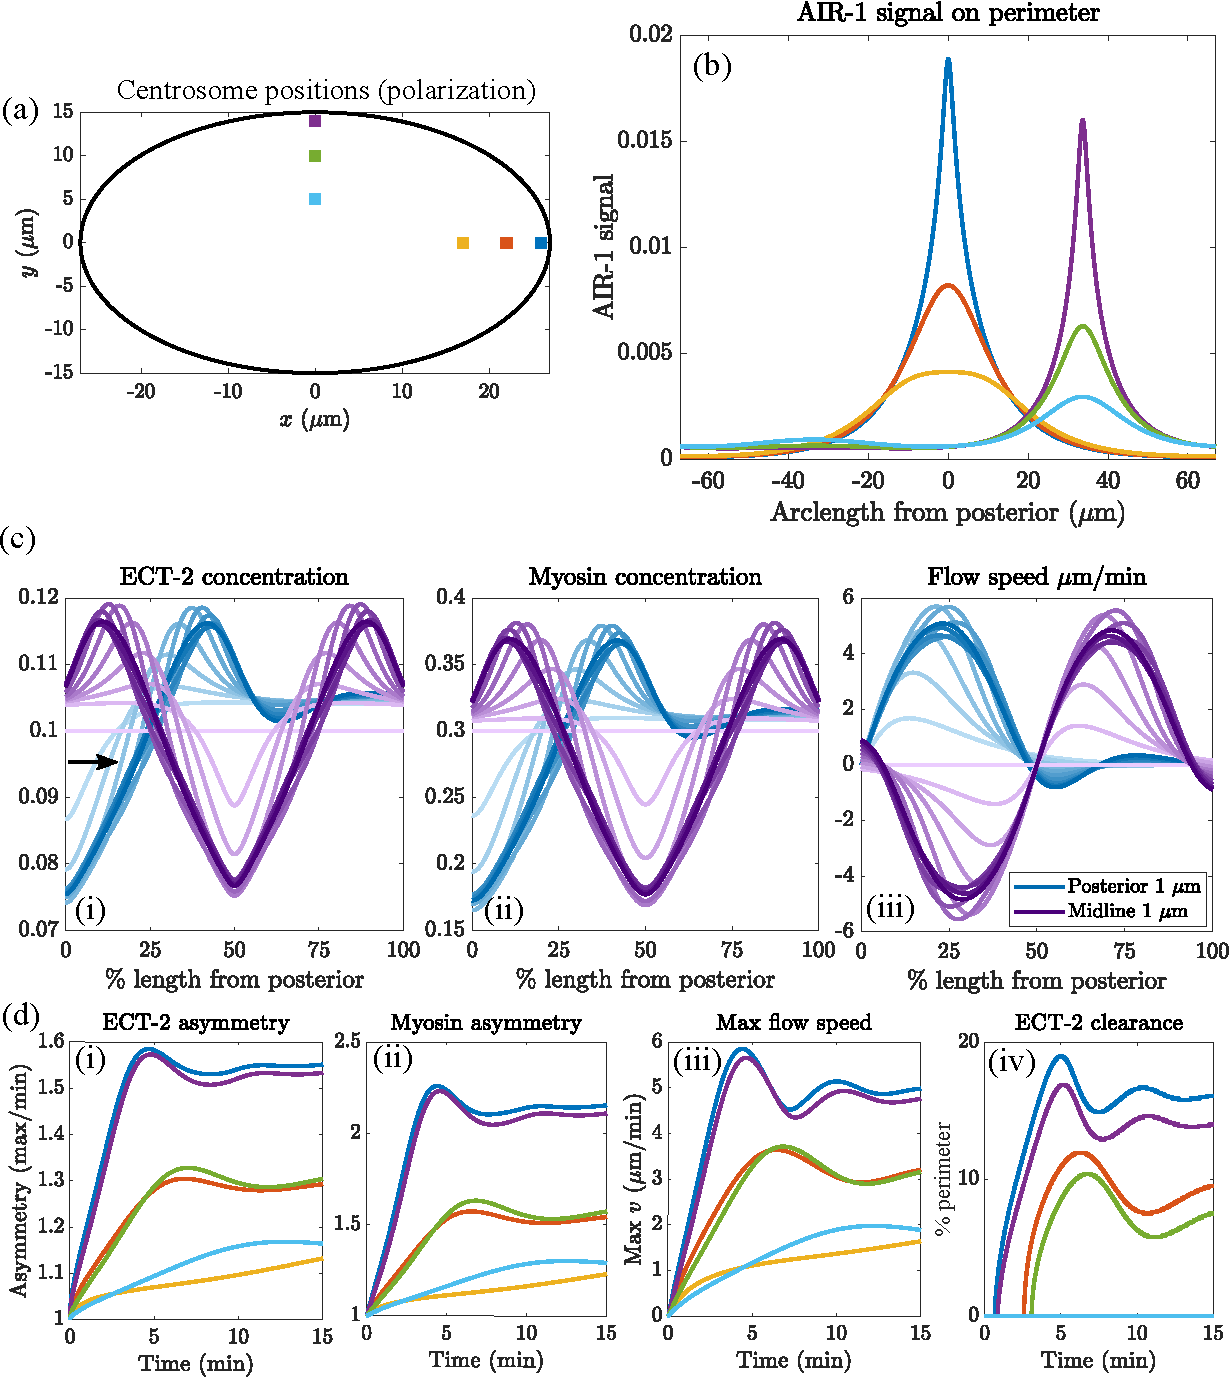
\includegraphics[width=\textwidth]{Glotzer/Fig5/Fig5-crop.pdf}
\caption{\label{fig:PolLoc}Centrosome locations set polarization dynamics. (a) The location of the centrosomes in our polarization simulations; we position both centrosomes 1, 5, and 10 $\mu$m away from the cell boundary on either the posterior pole or the cell midline. (b) The resulting AIR-1 signals along the cell perimeter. (c) The dynamics of polarization, starting from the uniform state, with the computed AIR-1 signal. Blue (purple) lines show the case when centrosomes 1 $\mu$m from the posterior pole (midline), and darker lines denote later times (0 to 10 mins). (d) Statistics on (i) ECT-2 asymmetry, (ii) myosin asymmetry, (iii) maximum flow speed, and (iv) ECT-2 clearance (measured as percentage of domain nearest the AIR-1 signal where the ECT-2 concentration is below 0.095 (see arrow in (c,i)) over time for the six centrosome locations shown in (a).}
\end{figure}

To explore the effect of centrosome distance and location, we position centrosomes at a distance 1, 5, and 10 $\mu$m from the posterior pole and cell midline, and measure the resulting AIR-1 signal. As shown in Fig.\ \ref{fig:PolLoc}(a,b), the AIR-1 signal is strongest in wild-type embryos (blue), where the curvature of the cell ``traps'' AIR-1 at the posterior pole. Because of effects of curvature, centrosomes positioned 1 $\mu$m from the cell midline have a smaller AIR-1 signal than those positioned 1 $\mu$m from the posterior pole, although the difference is at most 10--20\%. More drastic effects come when we move the centrosomes back from the cell boundary, with centrosomes 5 $\mu$m away giving a decrease of 50\% in AIR-1, and 10 $\mu$m giving an almost nonexistent AIR-1 signal.

Given these AIR-1 signals, we run the model (using the parameters obtained under cytokinesis conditions, with a slightly faster ECT-2 turnover in accordance with our FRAP experiments \citep[Fig.~3D]{longhini2022aurora}) forward in time to reach a steady state for polarization. Figure\ \ref{fig:PolLoc}(c) shows the trajectories of ECT-2, myosin, and the flow speed over time for signals aligned with the posterior pole and midline. Both signals exhibit roughly the same phenomena; there is a local clearing of ECT-2 and myosin near the centrosomes, which leads to a small peak roughly 35\% embryo length away from the signal position. This peak then flattens out as we move farther from the cue. Repeating these simulations for all centrosome positions gives the statistics shown in Fig.\ \ref{fig:PolLoc}(d). Under wild-type conditions, we predict an ECT-2 clearance (defined as the size of the region near the cue where $E < 0.095$; see the black arrow in Fig.\ \ref{fig:PolLoc}(c)) of about 17\% perimeter under wild type conditions, which translates to roughly 10 $\mu$m on either side of the pole, in good agreement with experimental observations in PAR mutants \citep[Fig.~2E]{gross2019guiding}. We also predict an A/P asymmetry of at most 1.5 during polarization, which matches what we observed in previously \citep[Fig.~1]{longhini2022aurora}, and a flow speed of at most 5--6 $\mu$m/min, which also matches observations in PAR mutants \citep[Fig.~2G]{gross2019guiding}. The time for peak clearance and asymmetries is delayed by about 1 minute when the centrosomes move from 1 to 5 $\mu$m from the cortex \citep[Fig.~3F]{bienkowska2012centrosomes}, and centrosomes 10 $\mu$m away give no clearance at all. Generally, centrosomes positioned at the posterior pole give faster flow speeds and higher clearances than those positioned at the midline, but the effect is slight. Considering that our results for ECT-2 clearance and asymmetry are in line with those determined experimentally, we conclude that the model we developed under cytokinesis conditions can also explain ``polarization'' in the absence of PAR proteins.


\subsection{Fast ECT-2 turnover and myosin recruitment gives robust polarization \label{sec:EctTurn}}

\begin{figure}
\centering
\includegraphics[width=\textwidth]{Glotzer/Fig6/Fig6-crop.pdf}
\caption{\label{fig:EctTurn}Alternative models show that ECT-2 turnover combined with myosin recruitment contributes to robust polarization dynamics. (a) A model where myosin no longer recruits ECT-2. Tuning parameters to get realistic flow speeds results in only marginal reorganization of ECT-2 (at most a 10\% difference). (b) Increasing the turnover time of ECT-2, so that it is advected by flows, leads to chaotic dynamics. Here we see that the lack of turnover leads to a sharp peak one hydrodynamic lengthscale away from the AIR-1 cue. In both cases, profiles are show every minute from $t=0$ to $t=10$ mins, with darker lines denoting later times.}
\end{figure}

We have shown that long-range reorganization of ECT-2 is possible despite its short residence time. The driver of this reorganization is recruitment by myosin, which is longer-lived on the cortex than ECT-2. Yet, is there any benefit to having rapid turnover of ECT-2 on the cortex? To explore this question, in Fig.\ \ref{fig:EctTurn} we consider two alternative models for polarization dynamics. In the first model, shown in Fig.\ \ref{fig:EctTurn}(a), we look at polarization when myosin no longer recruits ECT-2, changing parameters so that the flow is the same as that attained in PAR mutant embryos. With these realistic flow speeds, ECT-2 is not advected, and since it is not recruited by myosin, it cannot be transported over to the posterior. The result is an ECT-2 profile which is barely (at most 10\%) asymmetric. 

An obvious remedy to this problem is to increase the lifetime of ECT-2 on the cortex. In Fig.\ \ref{fig:EctTurn}(b), we increase the ECT-2 lifetime by an order of magnitude (from 2.5 s to 25 s), again tuning the flow speeds so that they are on the order 5 $\mu$m/min. We observe dynamics that are more chaotic. Initially (at $t=5$ mins), the ECT-2 and myosin distributions take on an asymmetry that matches that observed in Fig.\ \ref{fig:PolLoc}(c). After 5 minutes, however, the peak of myosin at 30\% length generates a strong flow which pulls ECT-2 from the posterior towards the anterior. This generates another minimum and a peak further towards the posterior, and we lose any notion of polarity.

Consider the situation at $t=5$ mins, where there is a small intermediate peak of ECT-2 and myosin. If ECT-2 is advected, it can be pulled into the peak from both sides, resulting in additional myosin and additional flows which increase the size of the peak. By contrast, if ECT-2 is not advected, flows alone cannot concentrate ECT-2 into peaks, and the flow coming from the anterior is driven primarily by a local equilibrium where ECT-2 is depleted because of the AIR-1 signal. This does not exist in the posterior, and so flows are negligible there (Fig.\ \ref{fig:PolLoc}(c)). These results demonstrate why a combination of rapid ECT-2 exchange and recruitment by myosin gives robust polarization with the experimentally-observed ECT-2 pattern and no large peaks. 

\subsection{A transient AIR-1 cue vs.\ local depletion}
\begin{figure}
\centering
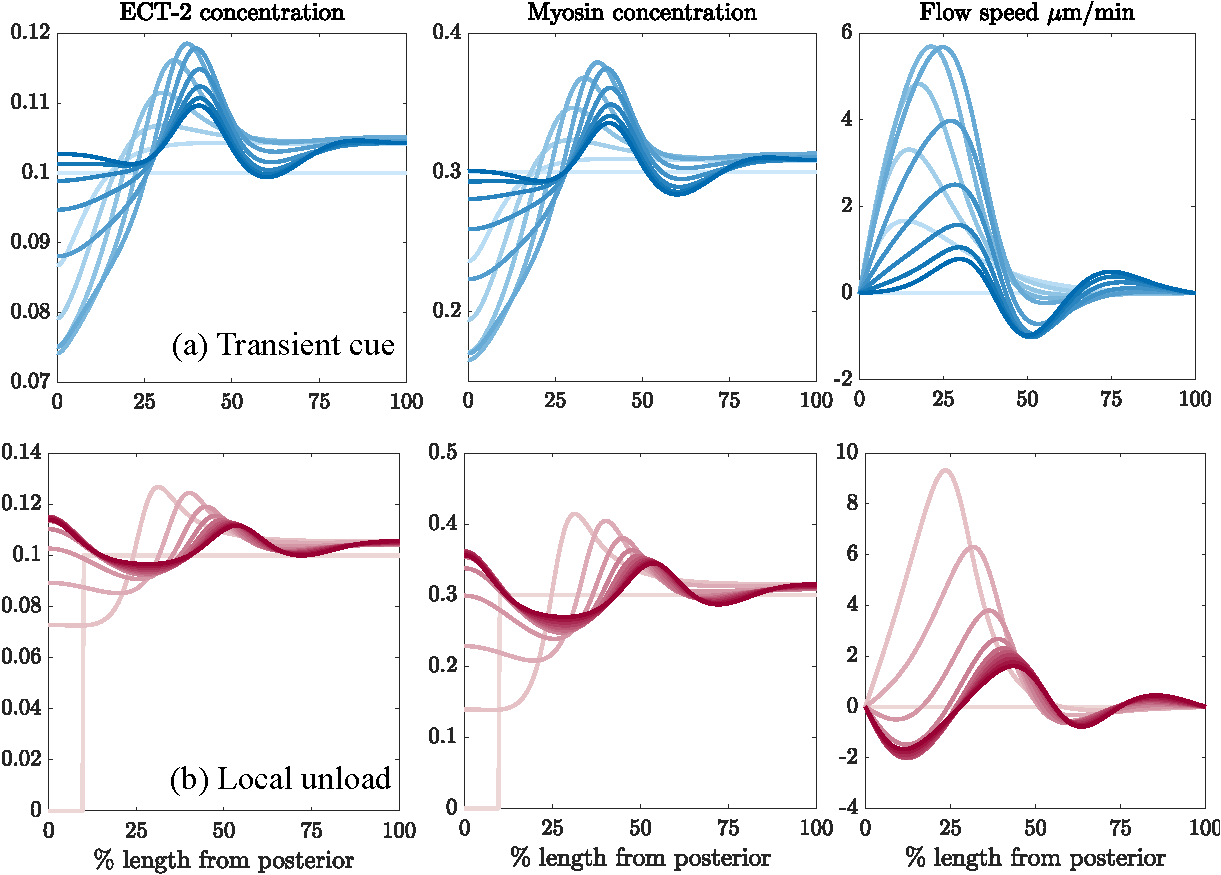
\includegraphics[width=\textwidth]{Glotzer/Fig7/Fig7-crop.pdf}
\caption{\label{fig:CueVsIC}Comparing a persistent (5 minute) AIR-1 cue to an initial condition of no myosin and ECT-2 at the posterior pole. (a) We simulate polarization with the AIR-1 cue in blue in Fig.\ \ref{fig:PolLoc} applied for five minutes, after which we remove the AIR-1 signal and watch relaxation. (b) There is no AIR-1 signal, but the initial condition has 10\% of the domain at an ECT-2 and myosin concentration of zero. As previously, we show profiles every minute from $t=0$ to $t=10$ mins., with darker lines denoting later times.}
\end{figure}

What is the difference between a transient AIR-1 cue and an initial local depletion of ECT-2 and myosin at the posterior pole? To answer this question, we perform two simulations: one with the AIR-1 cue (centrosomes 1 $\mu$m from the posterior pole) active for five minutes, and a second with no AIR-1 cue and an initial unloading of myosin and ECT-2 at the posterior pole. The resulting dynamics over ten minutes are shown in Fig.\ \ref{fig:CueVsIC}. For the transient AIR-1 cue, the flow starts at zero, and steadily increases over five minutes time to give a flow speed of 6 $\mu$m/min. Turning off the cue then brings the flow speeds below 2 $\mu$m/min in three minutes time. By contrast, unloading myosin and ECT-2 from the posterior at $t=0$ triggers a similar set of flows towards the anterior, but the flows are maximal at $t=1$ minute, and then steadily decrease over time. Experimental data in PAR mutants show flows which are at a maximum almost immediately after polarity triggering, but the magnitude (5 $\mu$m/min) of these flows persist throughout polarity establishment phase (3--4 mins) \citep[Fig.~2G]{gross2019guiding}. Thus, the true situation is likely a combination of local unloading and a persistent AIR-1 cue. 


\section{Dynamics of cytokinesis}
In previous work \citep{longhini2022aurora}, we collected a series of data on how the ECT-2 accumulation on the posterior/anterior cortex during cytokinesis depends on the position of the corresponding centrosomes. In \citep[Fig.~7A]{longhini2022aurora}, these are presented as individual embryos; here we average the individual embryos for each of the nine treatments and show the mean values (error bars are a single standard error in the mean) in Fig.\ \ref{fig:CytoSit}(a). We highlight two important aspects of this ``S-shaped'' curve: on both the anterior and posterior cortex, there is a plateau in the ECT-2 accumulation. That is, it appears that above or below a certain distance, the ECT-2 accumulation does not depend at all on the centrosome proximity. By contrast, for distances in the range 10--20 $\mu$m, there is an ultra-sensitive dependence of the ECT-2 concentration on the proximity. Our goal in this section is to use modeling to understand these trends.

\begin{figure}
\centering
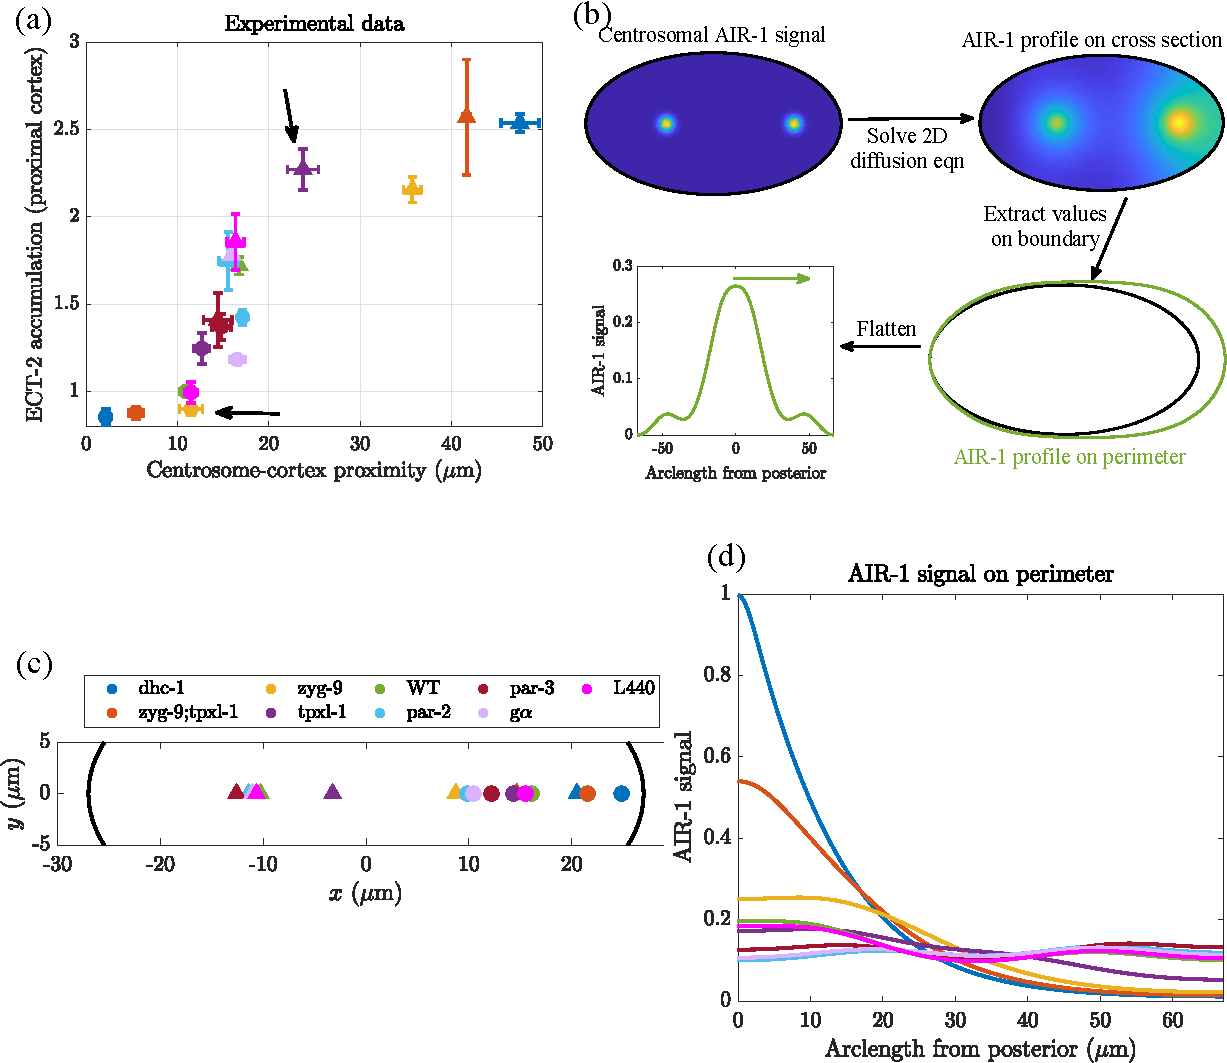
\includegraphics[width=\textwidth]{Glotzer/Fig2/Fig2-crop.pdf}
\caption{\label{fig:CytoSit} Modeling of AIR-1 signal in cytokinesis. (a) The experimental data for how the ECT-2 accumulation on the proximal cortex depends on the centrosome positions \citep[Fig.~7A]{longhini2022aurora}. Triangles are the anterior cortex, circles the posterior. Reproducing this plot via modeling is the central goal of this section. (b) Workflow for modeling the AIR-1 signal (in this case in wild-type embryos). (c) The centrosome positions for each embryo treatment, which are inputs to the diffusion model. (d) The corresponding AIR-1 signal on the cell perimeter, obtained from solving a diffusion equation. }
\end{figure}

\subsection{Solving for the AIR-1 profile}
In order to model the ECT-2 accumulation, we first need to use the centrosome locations to solve for the AIR-1 profile. Figure\ \ref{fig:CytoSit}(b) provides an overview of this process: for each embryo type, we obtain the centrosome positions, then solve a diffusion equation to obtain the AIR-1 profile on the entire embryo cross section. Evaluating the AIR-1 concentration (which has arbitrary units) on the boundary then gives a profile on the embryo perimeter, which we flatten out to a single periodic dimension. The mathematical details of this process are discussed in Appendix \ref{sec:AIR1D}; here it suffices to list the following assumptions that go into our model:
\begin{enumerate}[noitemsep, nolistsep]
\item During cytokinesis, the centrosomes have radius about 2 $\mu$m.
\item AIR-1 is activated on the centrosomes.
\item Active AIR-1 diffuses towards the cortex according to Fick's law.
\item A global phosphatase activity inactivates AIR-1 throughout the cytoplasm. 
\end{enumerate}
Setting the level of global phosphatase activity is a non-trivial undertaking. As shown in Appendix \ref{sec:AIR1D}, low levels of phosphatase activity give high global AIR-1 levels, which translate to low ECT-2 levels everywhere. Such levels were shown to block psuedocleavage in centralspindlin-independent cytokinesis, due to low contractility \citep{afshar2010regulation, kotak2016aurora}. Our choice is to set the phosphatase activity so that centrosomes close to the posterior pole (in polarization) have a negligible AIR-1 concentration in the anterior ($< 1\%$ of the anterior concentration).

Figure \ref{fig:CytoSit}(d) shows the AIR-1 signal (in arbitrary units) along the cell perimeter for each of the embryo treatments indicated in (c). We notice the high posterior levels of AIR-1 in dhc-1 (RNAi) and zyg-9;tpxl-1 embryos, which stand out from the rest. These same embryos have very low AIR-1 signals in the anterior (see Appendix \ref{sec:AIR1D}).

\subsection{Adding myosin-mediated flows reproduces the experimental trends}
\begin{figure}
\centering
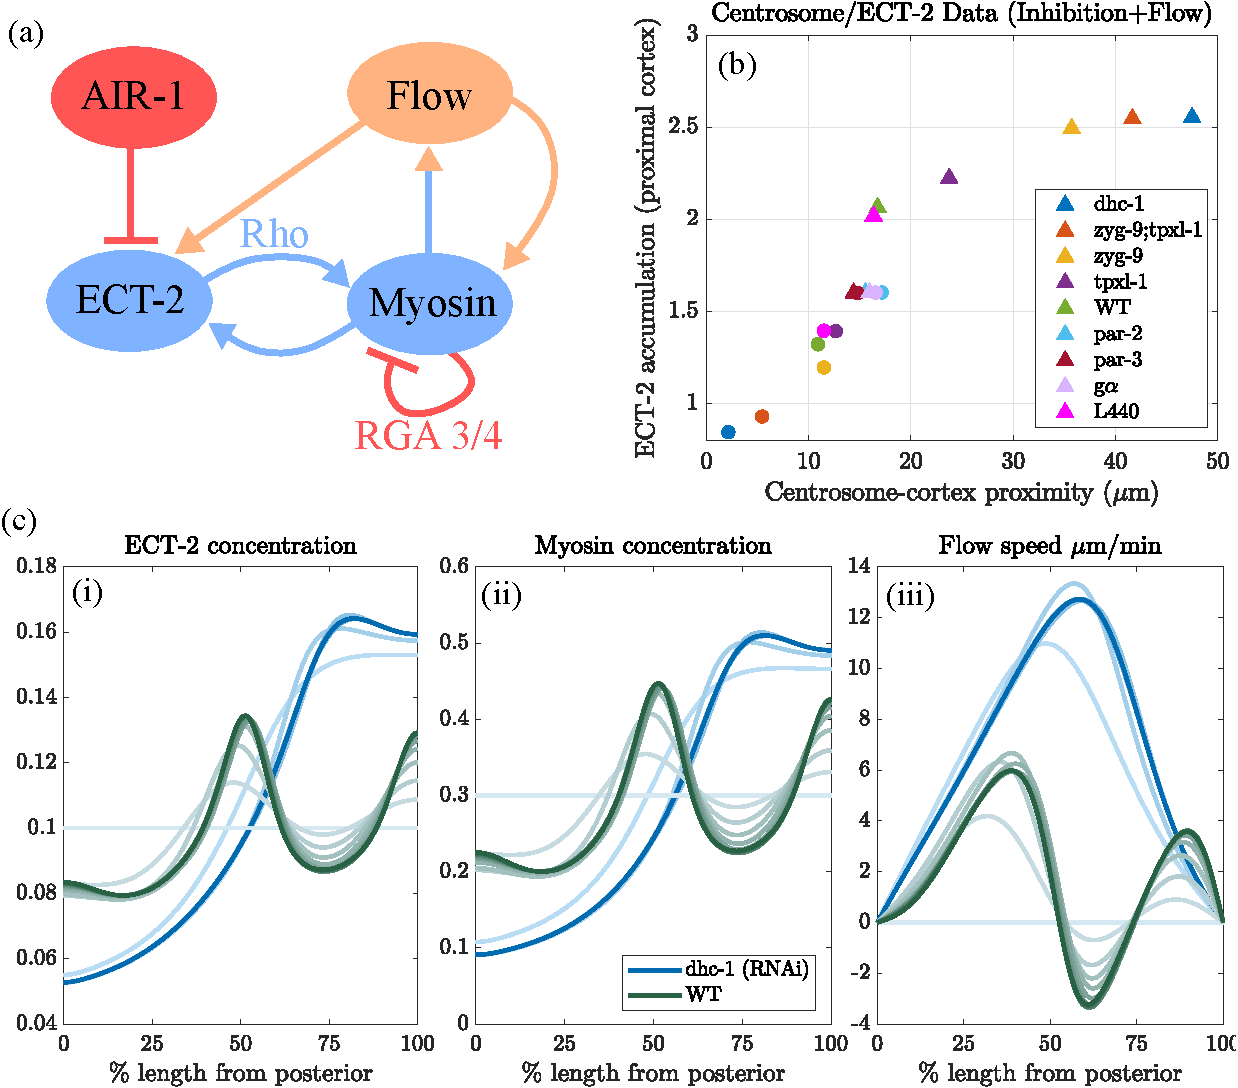
\includegraphics[width=\textwidth]{Glotzer/Fig4/Fig4-crop.pdf}
\caption{\label{fig:CytoWFlow}Incorporating flow into the AIR-1/ECT-2 model gives a better match to the experimental data. (a) Basic model of the ECT-2/Rho/Myosin circuit. (b) The corresponding data for ECT-2 accumulation vs.\ centrosome position (c.f.\ Fig.\ \ref{fig:CytoSit}(c)). (c) The dynamics of approach to steady state, starting from constant initial ECT-2 and myosin concentrations. Profiles of (i) ECT-2 concentration, (ii) Myosin concentration, and (iii) flow speed are shown from $t=0$ to $t=10$ mins, with snapshots shown every minute. Darker lines denote later times. Blue lines are dhc-1 (RNAi) embryos, while green lines denote WT. }
\end{figure}

Let us now consider a model, informed by the experimental data, by which asymmetries in AIR-1 could propagate through flows. The general schematic of our model is shown in Fig.\ \ref{fig:CytoWFlow}(a), and the mathematical details are presented in Appendix \ref{sec:MyModel}. The relationship between AIR-1 and ECT-2 is unchanged from \eqref{eq:EctASat}, but now the ECT-2 signal also activates myosin (through Rho), and myosin feeds back on ECT-2 through direct recruitment, and through advection by flows. Finally, there is delayed negative feedback of myosin accumulation (through RGA-3/4-dependent inactivation of RHO-1) \citep{michaux2018excitable}. To constrain unknown model parameters, we assume that 
\begin{enumerate}[noitemsep, nolistsep]
\item 10\% of ECT-2 is bound to the cortex at steady state in wild-type embryos (our own unpublished(?) measurements). 
\item 30\% of myosin is bound to the cortex at steady state in wild-type embryos \citep[Fig.~S3j]{gross2019guiding}.
\item There is a modest increase (two-fold) in the recruitment rate of ECT-2 due to cortial myosin, in a myosin concentration-dependent manner.
\end{enumerate}
As dicussed in Appendix \ref{sec:MyModel}, these assumptions are sufficient to constain all but two of the model parameters. The two parameters that remain describe the strength of myosin flows and the strength at which AIR-1 inhibits ECT-2. We have already seen the case when the latter is high and the former is zero (Fig.\ \ref{fig:LinFail}(b)). In order to match the experimental data while keeping the A/P ratio in dhc-1 embryos constant, we systematially decrease the AIR-1 inhibition strength and increase the speed of flows until we get dynamics which resemble the experimental data in both wild type and dhc-1 (RNAi) embryos. With the parameters chosen, AIR-1 increases the off rate of ECT-2 by about 50\% in the posterior of dhc-1 embryos, and in wild-type embryos AIR-1 increases the off~rate of ECT-2 by 30\% in the posterior and 20\% in the anterior.

Figure \ref{fig:CytoWFlow}(c) shows the model's approach to steady state (over 10 minutes of simulation time from an initially uniform state) in both dhc-1 (blue) and wild type (green) embryos. With the chosen parameters for inhibition strength and flow speed, the flows are of a realistic magnitude, and the ECT-2 concentration ratios between the anterior and posterior poles resemble the experimental measurements. Fig.\ \ref{fig:CytoWFlow}(b) shows the ECT-2 accumulation on the anterior/posterior pole across all embryo treatments, taken at the time of maximum asymmetry. We observe a plateau at the low end, corresponding to saturation of the AIR-1 signal, and a plateau at the high end, where myosin accumulation and flow is inhibited by RGA 3/4. In the middle, we see an ultra-sensitive dependence: moving from 10--20 $\mu$m centrosome distance gives a roughly two-fold change in ECT-2 accumulation, similar to the experimental data in Fig.\ \ref{fig:CytoSit}(a). 



\section{Discussion}

\begin{appendix}
\section{Mathematical appendix} 

\subsection{AIR-1 diffusion model \label{sec:AIR1D}}
The contractility circuit is forced by a cue from the centrosomes which contain Aurora A (AIR-1), an inhibitor of ECT-2. We assume that the AIR-1 signal gets to the membrane by diffusion. Letting $a(\V x)$ be the concentration of AIR-1 in the two-dimensional embryo cross-section, we have the equation
\begin{subequations}
\label{eq:CD}
\begin{align}
\label{eq:DiffEqn}
\Delta a -\koffb a=  -f \qquad &\V{x} \in \Omega.\\
\label{eq:DiffBC}
\nabla a \cdot \V{n}=0 \qquad &\V{x} \in \partial \Omega,
\end{align} 
where\ \eqref{eq:DiffEqn} is the diffusion equation for the concentration and\ \eqref{eq:DiffBC} is a no-flux boundary condition through the boundary (here $\Omega$ represents the embryo area and $\partial \Omega$ represents the boundary). The signal $f(\V x)$ comes from the two centrosomes, which we model by Gaussian densities 
\begin{equation}
f(\V{x}) = \frac{C_0/D}{2 \pi \sigma_c^2}\sum_{i=1}^2\exp{\left(\frac{-\norm{\V{x}-\V{x}_i}^2}{2 \sigma_c^2}\right)}.
\end{equation}
Here $\V{x}_i$ is the location of the $i$th centrosome (typically at some location $(x_i,0)$), which changes depending on the embryo conditions. In addition to the centrosome location, the signal has two other parameters: $C_0/D$ is the strength of the cue (the integral of $f(\V{x})$ over the entire embryo cross-section, normalized by the cytoplasmic diffusion coefficient $D$), and $\sigma_c$ is the centrosome ``size'' (the standard deviation of the Gaussian, which is roughly half the size of the centrosome). For cytokinesis, the centrosomes have size about 2 $\mu$m, so we set $\sigma_c=1$ $\mu$m. In polarization, the centrosomes have size about 0.2 $\mu$m, so we set $\sigma_c=0.1$ $\mu$m. The signal strength $C_0/D$ is arbitrary; we set it to 1 for cytokinesis and 0.01 for polarization, thus assuming that the total amount of AIR-1 signal is proportional to centrosome area.
\end{subequations}
The diffusion equation\ \eqref{eq:DiffEqn} also contains a basal rate of inactivation of AIR-1 (phosphatase activity). This introduces another parameter which is the inactivation rate relative to the diffusion coefficient in the cytoplasm ($\koffb$, units $\mu$m$^{-2}$). 

We use a standard first-order finite element method to solve\ \eqref{eq:DiffEqn}. In brief, the elliptical domain of the embryo is meshed into nodes and triangles \citep{persson2004simple}, which define a set of linear Lagrangian basis functions $\psi_k$ that are 1 at node $\V{x}_k$ and 0 everywhere else. Multiplying\ \eqref{eq:DiffEqn} by a basis function $\psi_k$, then integrating by parts using the boundary condition\ \eqref{eq:DiffBC} gives 
\begin{equation}
\sum_j \int_{\Omega} \left(\nabla \psi_k \cdot \nabla \psi_j\right) a_j \, d\V{x}+\sum_j \int_{\Omega} \psi_k \psi_j a_j \, d\V{x}= \sum_j \int_{\Omega} \psi_k \psi_j f_j \, d\V{x},
\end{equation}
which can be written as the matrix equation $\left(\M K + \koffb \M M \right) \V a = \M M \V f$, where $\M{M}$ is the so-called mass matrix and $\M{K}$ the stiffness matrix for finite elements. These matrices are assembled using standard techniques \citep[c.~7]{gockenbach2006understanding}; see the github repository \url{https://github.com/omaxian/CElegansModel/} for code.

\subsection{ECT-2/Myosin circuit \label{sec:MyModel}}
We here formulate the equations for the model shown in Fig.\ \ref{fig:CytoWFlow}(a), where ECT-2 (through activating $\rho$) activates myosin at the cortex. To minimze the number of parameters, we consider a simplified version of the true dynamics (where ECT-2 signals myosin by activating rho) and formulate a model with two variables, $E$ (for ECT-2) and $M$ (for myosin). In dimensional units (denoted by hats), the equations we use are 
\begin{subequations}
\label{eq:MyDim}
\begin{gather}
\partial_{\hat t} \hat E + \partial_{\hat x} \left( \hat v \hat E\right) = \hat D_E \partial_{\hat x}^2 E +\kon_E \left(1+k_\text{ME} \hat M\right)\hat E_c - \koff_E  \left(1+k_\text{AE}\left( \frac{\hat A}{\hat A_c+\hat A}\right)\right)\hat E \\
\partial_{\hat t} \hat M +\partial_{\hat x} \left( \hat v \hat M\right)  = \hat D_M \partial_{\hat x}^2 M +k_\text{EM} \hat E ^2 \hat M_c - \koff_M \hat M -k_\text{fb} \hat M^4 \\
\label{eq:veleqn}
\gamma \hat v = \eta \partial_{\hat x}^2 \hat v +\hat \sigma_0 \partial_{\hat x} \hat M \\
\label{eq:CytoDim}
\hat E_c = \frac{1}{hL}\left(\Tot{E}L-\int_0^L \hat E(\hat x) \, d\hat x\right), \qquad \hat M_c =\frac{1}{hL}\left(\Tot{M}L-\int_0^L \hat M(\hat x) \, d \hat x\right).
\end{gather} 
\end{subequations}
Each of the species ECT-2 and myosin evolves by
\begin{enumerate}[noitemsep, nolistsep]
\item \emph{Advection by cortical flows.}  These are the terms $\Dx (v E)$ and $\Dx (v M)$.
\item \emph{Diffusion in the cortex.} These are the terms $D_E \Dx^2 E$, and $D_M \Dx^2 M$.
\item \emph{Binding to the cortex.} For ECT-2, there is a basal binding rate plus a linear enhancement by myosin. For myosin, the binding rate is proportional to the square of the ECT-2 concentration, without a basal binding rate. The motivation for this term is that myosin asymmetries are typically much stronger than ECT-2 asymmetries \citep{longhini2022aurora, munro2004cortical, mayer2010anisotropies}, and thus some nonlinearity is required. We choose the minimal such nonlinearity (see \citep[Eq.~(1)]{michaud2022versatile} for another choice, where Rho is represented explicitly). The binding rate is also proportional to the cytoplasmic concentration of each protein, defined in\ \eqref{eq:CytoDim}, where $L$ is the domain length, $h$ is the cytoplasmic ``thickness'' (so that $hL$ is the total area), and $\Tot{A}$ is the concentration of protein $A$ when all of it is bound to the cortex \citep{lang2022oligomerization}.
\item \emph{Unbinding from the cortex.} For ECT-2, the unbinding rate is composed of a basal rate expressing the fast exchange of ECT-2, plus inhibition by AIR-1 according to\ \eqref{eq:EctASat}. Myosin unbinds with a basal rate (expressing the combination of inactivation and unbinding), which is enhanced by delayed negative feedback (the $M^4$ term). The form of this term is a coarse-grained version of previously-published work \citep{michaux2018excitable}. The model there considered rho ($\rho$) and RhoGAP ($r$) as the unknowns, with the production of RhoGAP proportional to $\rho^3$ and the inhibition of $\rho$ proportional to $r \rho/(K+\rho)$. Here we coarse-grain this model into a single term, with the inhibition proportional to $M^4$. 
\end{enumerate}
Finally, the velocity equation \eqref{eq:veleqn} expresses the balance of active stress (which we assume is proportional to myosin concentration) with viscous stress and frictional resistance \citep{mayer2010anisotropies}. 

\subsubsection{Non dimensionalization}
Because absolute concentrations are unknown, it is easiest to assign values to unknown parameters when they are in dimensionless form. To do this, we non-dimensionalize so that length is in units of the embryo perimeter $L$, time is in units of the bound myosin lifetime $1/k^\text{off}_M$, velocity is in units of $\sigma_0/\left(\sqrt{\eta \gamma}\right)$ \citep{bois2011pattern} and concentration of species $A$ is in units of $\Tot{A}$. This gives new dimensionless variables 
\begin{subequations}
\label{eq:MySimple}
\begin{equation}
\label{eq:NDD}
x = \hat{x}/ L \qquad t=  \hat t \koff_M \qquad M= \hat{M}/\Tot{M}  \qquad E= \hat{E}/\Tot{E} \qquad v = \hat{v}/\left( \frac{\hat \sigma_0}{\sqrt{\eta \gamma}}\right),
\end{equation}
and a corresponding set of equations
\begin{gather}
\Dt E + \sigma_0 \Dx \left( v E\right) = D_E \Dx^2 E +\Kon_E \left(1+\Kme M\right)E_c - \Koff_E  \left(1+\Kae \left(\frac{A}{A_c+A}\right)\right)E \\
\label{eq:MyEq}
\Dt M + \sigma_0 \Dx \left( v M \right) = D_M \Dx^2 M +K_\text{EM} E ^2M_c - M -\Kfb M^4 \\
\label{eq:veleqn}
v = \ell^2 \Dx^2 v +\ell \Dx M \\
E_c = 1-\int_0^1 E(x) \, dx \qquad M_c = 1-\int_0^1 M(x) \, dx.
\end{gather} 
The conversion from dimensional to dimensionless form is straightforward for most of these parameters. Since some (e.g. $\Kae$, $\Kme$) are unknown anyway, it is not useful to report how they relate to the dimensional parameters. There are some important parameters to highlight, however. In flow patterns, $\ell=\left(\sqrt{\eta/\gamma}\right)/L$ is a hydrodynamic lengthsale (scaled by domain perimeter) expressing the connectivity of the cortex; local disturbances in myosin will typically propagate at most a distance $\ell$. The parameter $\sigma_0 = \hat \sigma_0/\left(L\koff_M \sqrt{\eta \gamma}\right)$ expresses the strength of the flows; the dimensional velocity in $\mu$m/s can be extracted by taking $v \times \sigma_0 L \koff_M$. 

\end{subequations}


\subsubsection{Parameter estimation}
A simple set of assumptions, some of which are based on experimental data, allows us to reduce the dynamics in\ \eqref{eq:MySimple} to two unknown parameters. We do this as follows, 
\begin{enumerate}[noitemsep, nolistsep]
\item The embryo cross section is an ellipse with approximate radii 27 $\mu$m and 15 $\mu$m, which gives a perimeter $L=134.6$ $\mu$m \citep{goehring2011polarization} .
\item The variable $\ell$ is the hydrodynamic lengthscale. In dimensional units, this was measured to be approximately 13 $\mu$m \citep{mayer2010anisotropies}, which means $\ell = 0.1$ in \eqref{eq:MySimple} (10\% domain length).  
\item The myosin bound lifetime is about 15 s, so $\koff_M=1/15$ s$^{-1}$.
\item We assume that all species have a dimensional diffusion coefficient $\hat D_{E/M}=0.1$ $\mu$m$^2$/s \citep{goehring2011polarization, gross2019guiding, robin2014single}. Rescaling length by $L$ and time by $\koff_M$ gives a dimensionless coefficient $D_E=D_M=0.1/(L^2 \koff_M)=4.6 \times 10^{-5}$. 
\item The ECT-2 lifetime was measured using FRAP to be on the order of a few seconds \citep[Fig.~3D]{longhini2022aurora}. In cytokinesis, we set $\koff_E=0.33$/s, for a three second lifetime. Rescaling gives $\Koff_E=\koff_E/\koff_M=5$. Our data shows slightly faster recovery during polarization, so we increase $\koff_E$ by 20\% for those simulations.
\item The value of $\Kme M$ determines what fraction of ECT-2 binding occurs from recruitment by myosin. We assume that 50\% of ECT-2 is recruited by myosin, so that $\Kme M = 1$. Because $M \approx 0.3$ (see assumption 7), we set $\Kme=1/0.3$. 
%\item The value of $\Kem E$ determined what fraction of myosin activation occurs via the ECT-2 pathway. We assume that 2/3 of myosin is activated by ECT-2, so that $\Kem E=2$. Because $E \approx 0.1$ (see assumption 7), we set $\Kem=20$. 
\item In wild type embryos at steady state, we assume that 10\% of ECT-2 is bound to the cortex (our own unpublished(?) data), and 30\% of myosin is bound to the cortex \citep[Fig.~S3j]{gross2019guiding}. This sets $\Kon_E=0.34$ and $\Kem = 50$. 
\item For the negative feedback of myosin, we use the parameters determined in \citep{michaux2018excitable}. The feedback strength is obtained by assuming an equilibrium of RhoGAP in the equations of \citep{michaux2018excitable} (neglecting the basal binding rate), which gives (in their notation) $\Kfb=k_\text{GAP}\left(k_r^\text{ass}/k_r^\text{diss}\right)=0.1(0.245/0.047)=0.52$/s. Rescaling by $\koff_M$ gives $\Kfb=7.8$ in our model. 
\item According to our experimental data in Fig.\ \ref{fig:CytoSit}, the effect of the AIR-1 signal should saturate around $A \approx 0.2$. We therefore set $A_c=0.2$. 
\end{enumerate}
This systematic fitting procedure reduces the dynamics to two parameters: $\Kae$, which describes the rate at which AIR-1 inhibits ECT-2, and $\sigma_0$, which is the speed of flows induced by myosin gradients. By manipulating these two parameters, we can model situations where ECT-2 gradients are due to AIR-1 alone ($\sigma_0 = 0$), or where there is substantial amplification by flows (small $\Kae$). In the extreme case when $\Kae=0$ and $\sigma_0$ is sufficiently large, we will get oscillatory dynamics, with peaks of myosin occuring at random places, in accordance with the model of \citep{michaux2018excitable}. We need a sufficiently large $\Kae$ to ensure that the myosin peaks correspond to locations of AIR-1 depletion.

Our approach is to start with a uniform concentration of ECT-2 and myosin, then apply the AIR-1 signal and watch the dynamics for ten minutes (long enough to reach a rough steady state, as shown in Fig.\ \ref{fig:CytoWFlow}). To find a combination of $\Kae$ and $\sigma_0$ that best satisfies the data, we start by fixing $\Kae$, then adjust $\sigma_0$ so that dhc-1 embryos have the experimental A/P ratio ($\approx 3.2$) of ECT-2 at steady state. We accept a pair of parameters $\left(\Kae,\sigma_0\right)$ if these same parameters give an A/P ratio around 1.7 in wild-type embryos as well. Figure\ \ref{fig:CytoWFlow} shows the dynamics over ten minutes with our chosen parameters $\Kae=0.6$ and $\sigma_0=0.2$. Note that $\Kae=0.6$ implies that AIR-1 is increasing the off-rate of ECT-2 by about 50\% in the posterior of dhc-1 (RNAi) embryos ($A \approx 1 \rightarrow \Kae A/(A+A_c) \approx 0.5$), and 30\% in the posterior of wild-type embryos ($A \approx 0.2 \rightarrow \Kae A/(A+A_c) \approx 0.3$).

\subsubsection{Numerical solution}
We use standard numerical methods to solve \eqref{eq:MySimple}. We discretize the one-dimensional domain at $N$ points with spacing $1/\Delta x$, and define the centered differentiation matrix $\M{D}$ and standard three points Laplacian differentiation matrix $\M{\Delta}$. Given the myosin profile at time step $n$, we first compute the velocity $v^{(n)}$ by solving $v^{(n)} = \ell^2 \M{\Delta} v^{(n)} + \ell \M{D} M^{(n)}$. Once the velocity is computed the ECT-2 and myosin equations are solved by combining a first-order upwind finite volume scheme for the advection terms \citep[Sec.~1.4]{hundsdorfer2003numerical} with implicit treatment of the diffusion terms (using the standard three point Laplaian). The reaction terms are all treated explicitly, and time-stepping is first order accurate. Matlab code  is available at the github repository \url{https://github.com/omaxian/CElegansModel/}.

\subsubsection{Parameter adjustments: polarization \label{sec:EctTurnP}}
In Section \ref{sec:EctTurn}, we modify the parameters to examine alternative hypotheses for the dynamics of polarization. We first consider what happens if ECT-2 is not recruited by myosin, in which case we adjust the on rate to $\Kon_E=0.68$ and $K_\text{ME}=0$. The flows are adjusted to 5 $\mu$m/min by setting $\sigma_0=0.5$. 

Another alternative is that ECT-2 has a longer lifetime and can be advected by flows this way. We consider in particular $\koff_E=1/25$ s$^{-1}$ (25 s residence time instead of 2.5) and $\Kon_E=0.068$ to give a 10\% bound ECT-2, and $K_\text{ME}=0$, so that myosin doesn't recruit ECT-2. All other parameters take their default values (in particular, $\sigma=0.2$ again). 

\section{Supplemental investigations and figures}
\subsection{Cortex model validation and parameter selection}
This shows that the myosin terms and $\Kem$ is correct. \red{Still need validation for $\Kme$.}

\begin{figure}
\centering
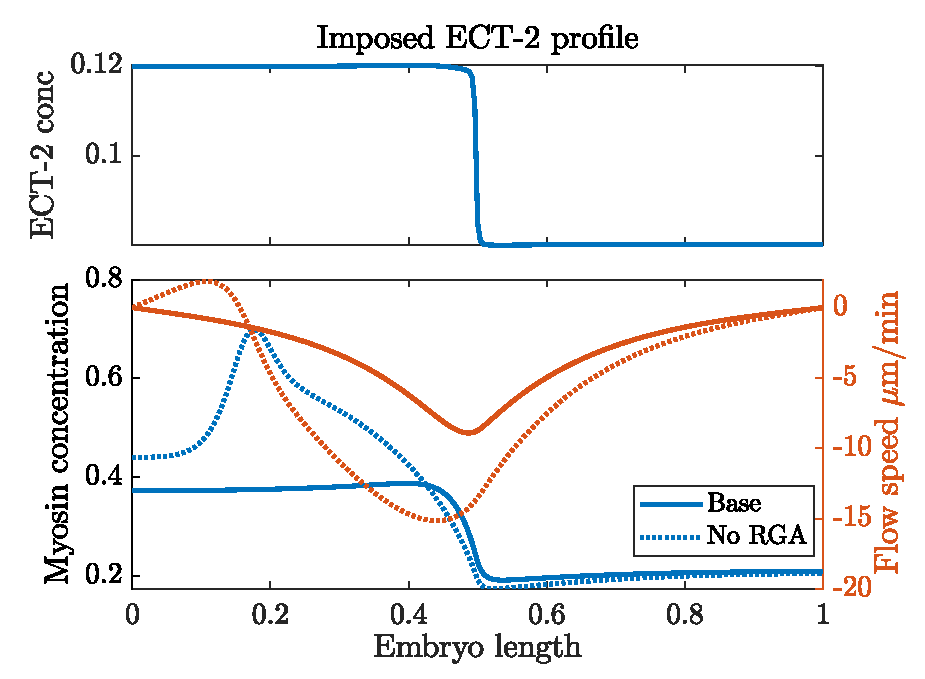
\includegraphics[width=0.6\textwidth]{ModelCheckRGA.eps}
\caption{\label{fig:CortexMod}Validating our simple model of the cell cortex. We fix the ECT-2 profile and perform simulations with (solid lines) and without (dotted lines) the myosin negative feedback term $\Kfb M^4$ in\ \eqref{eq:MyEq}. }
\end{figure}

\subsection{Constraining level of AIR-1 phosphatase activity}
To constrain the level of phosphatase activity (parameter $\koffb$), we compute the profile of AIR-1 under polarization conditions (both centrosomes 1 $\mu$m from the posterior pole, with $C_0/D=0.01$), and plot the resulting AIR-1 signal in Fig.\ \ref{fig:AIR1ProfKoff}. When the phosphatase activity is low, the no flux boundary condition traps AIR-1 inside the embryo, and the relative difference between posterior and anterior is small. Increasing the phosphatase activity disproportionately lowers AIR-1 levels on the anterior pole (since it is much farther from the centrosomes). We assume that anterior levels of AIR-1 during polarization are at most 1\% of posterior levels; this constrains $\koffb=10^{-2}$. 

\begin{figure}
\centering
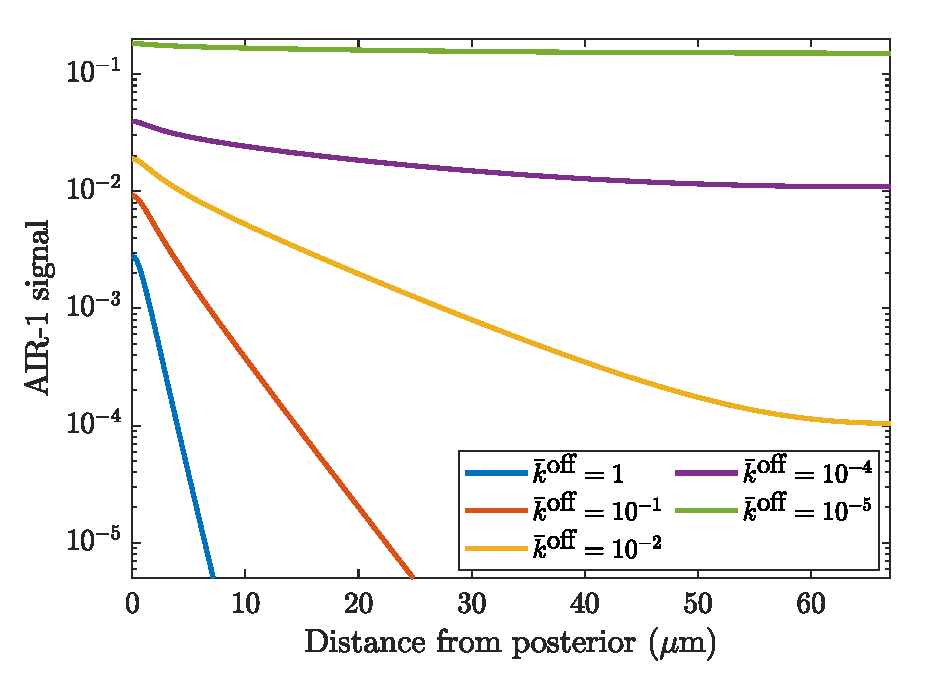
\includegraphics[width=0.6\textwidth]{Glotzer/PolarizationKoffAir.eps}
\caption{\label{fig:AIR1ProfKoff}AIR-1 signal vs.\ distance from posterior under polarization conditions (blue squares in Fig.\ \ref{fig:PolLoc}(a)). We vary the level of phosphatase activity $\koffb$ until the posterior level is less than 1\% of the anterior level, settling on $\koffb=10^{-2}$ $\mu$m$^{-2}$.}
\end{figure}


\subsection{Myosin-independent models for the ECT-2 response are inadequate}
In the simplest possible model of ECT-2 dynamics, there is a local equilibrium of the binding rate and unbinding rate, where the latter increases in the presence of AIR-1,
\begin{equation}
\label{eq:EctA}
 \kon_E = \koff_E \left(1+\Kae A \right)E,
\end{equation}
and $\Kae$ expresses the strength of inhibition. This steady state model predicts that the ECT-2 concentration relates to the AIR-1 concentration at the cortex via
\begin{equation}
\label{eq:EctLinA}
E = \frac{\kon_E/ \koff_E}{ 1+\Kae A},
\end{equation}
which is a relationship with two unknown constants. Fitting these two unknown constants to the observed ECT-2 levels in dhc-1 (RNAi) embryos (where the AIR-1 signal is approximately 1 at the posterior and 0 at the anterior) gives $\kon_E/ \koff_E=2.55$ and $\Kae=2$. Substituting the AIR-1 levels from the other embryo treatments then gives the observed centrosome/ECT-2 accumulation plot shown in Fig.\ \ref{fig:LinFail}(a). There we see that the relationship \eqref{eq:EctLinA} correctly predicts saturation at low levels of AIR-1 (high centrosome-cortex distances), but fails to predict saturation at high AIR-1 levels (low distances) or ultra-sensitivity in between. 

\begin{figure}
\centering
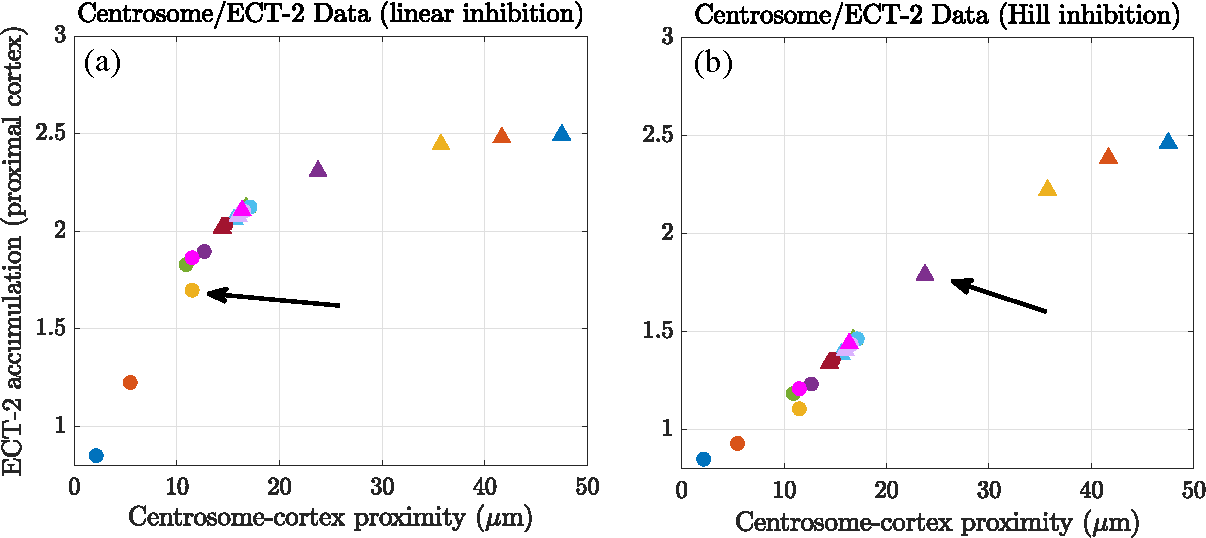
\includegraphics[width=\textwidth]{Glotzer/Fig3/Fig3-crop.pdf}
\caption{\label{fig:LinFail}Simple models based on AIR-1/ECT-2 inhibition fail to capture the experimental data on accumulation vs.\ centrosome position. We consider (a) a linear inhibition model \eqref{eq:EctLinA}, and (b) a linear model with saturation \eqref{eq:EctASat} (Hill function). Compared to the data in Fig.\ \ref{fig:CytoSit}, neither of these simple models capture the general S-shape of the curve, with plateaus at the low and high ends. }
\end{figure}

The AIR-1 signals we obtained in Fig.\ \ref{fig:CytoSit}(d) show that the AIR-1 signal at the posterior doubles when we switch from zyg-9;tpxl-1 (red) embryos to dhc-1 embryos (blue). Yet, the experimental data in Fig.\ \ref{fig:CytoSit}(a) show that the ECT-2 accumulation is unchanged. This tells us that there must be saturation in the AIR-1 inhibition dynamics; beyond some level, the amount of AIR-1 no longer impacts the inhibition strength. Based on the location of the plateau in the experimental data, it seems that this threshold level occurs around the posterior AIR-1 level in zyg-9 embryos, which our data in Fig.\ \ref{fig:CytoSit}(d) tells us is 0.2. Thus, we propose a new model where the local equilibrium is governed by 
\begin{equation}
\label{eq:EctASat}
 \kon_E = \koff_E \left(1+\Kae \left(\frac{A}{A_c+A}\right) \right)E,
\end{equation}
where $A_c=0.2$. Once again fitting $\kon_E/\koff_E=2.8$ and $\Kae=2.8$ to the data for dhc-1 embryos, we obtain the centrsome/ECT-2 plot shown in Fig.\ \ref{fig:LinFail}(b). There we see that we have correctly reduced the posterior ECT-2 levels in embryos with high AIR-1 signals to approach a plateau. However, we also reduce the ECT-2 levels in the other embryos (especially tpxl-1; purple), and we still no longer see the ulta-sensitivity in distances 10--20 $\mu$m. We propose that the failure of these simple models comes from a lack of propagation of the AIR-1/ECT-2 signal via flows. If flows can exaggerate the smaller  asymmetries in a manner proportional to the AIR-1 signal, we might be able to reproduce the experimental data.


\end{appendix}

\bibliographystyle{plainnat}

\bibliography{../../PolarizationBib}


\end{document}
